\chapter{Concordances}

We have prepared our corpus and now it is time to visualize it.\marginnote{Visualizations in Orange are designed to support selection and passing of the data that applies to it. Finding interesting data subsets and analyzing their similarities is a central part of exploratory data analysis.} We have already seen some of the preprocessing results in a word cloud. But we still don't know much about the use of a specific word in a text. Since we lowercased the text, there might be some conflation. For example 'oh' could be a lowercase version of OH (the chemical compound of hydroxide), a simple exclamation 'Oh!' or an abbreviation for the state of Ohio.\marginnote{To inspect the documents containing a particular word, select the documents in Concordance and pass them to Corpus Viewer for a deeper analysis.}

To check the context of a particular word we can use Concordance widget. Concordance shows us the text around our word.

Connect \widget{Concordance} to \widget{Corpus} to pass the text to the widget. To browse the word, type it in the query line at the top or provide it with the \widget{Word Cloud}. Here we have selected the word 'king' in the Word Cloud and observed the context in Concordance.

\vspace{-0.2cm}
\begin{figure}[h]
  \centering
  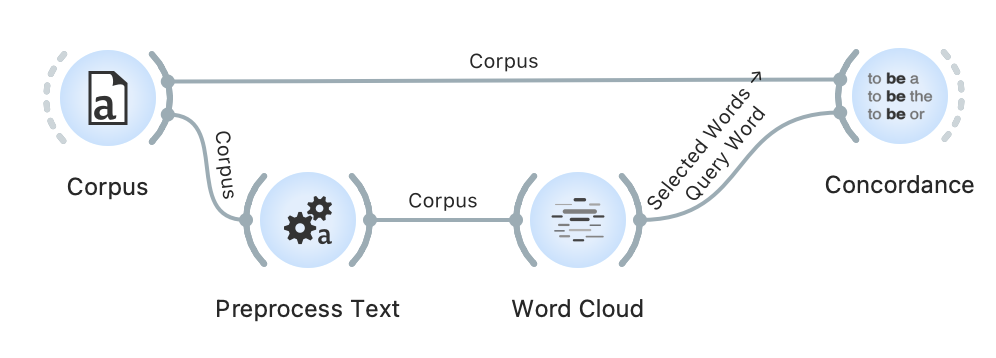
\includegraphics[width=\linewidth]{workflow.png}%
  \caption{$\;$}
\end{figure}
\vspace{-0.3cm}

\begin{figure*}[h]
    \centering
    \infinitewidthbox{
      \stackinset{r}{-0.35\linewidth}{t}{+0.1\linewidth}
      {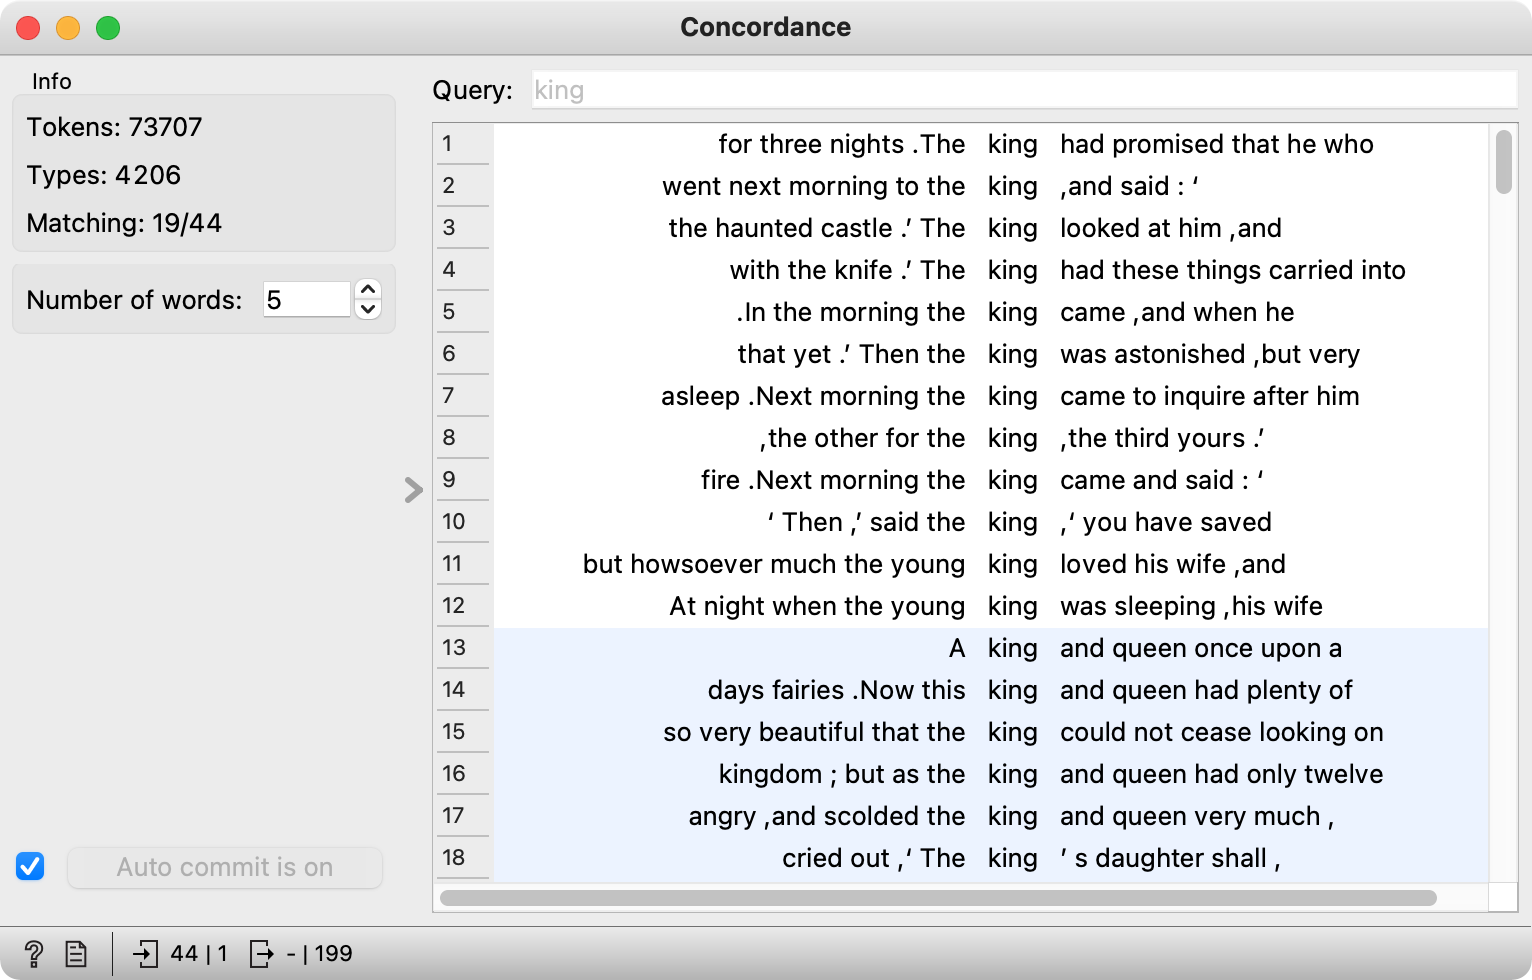
\includegraphics[scale=0.35]{concordance.png}}
      {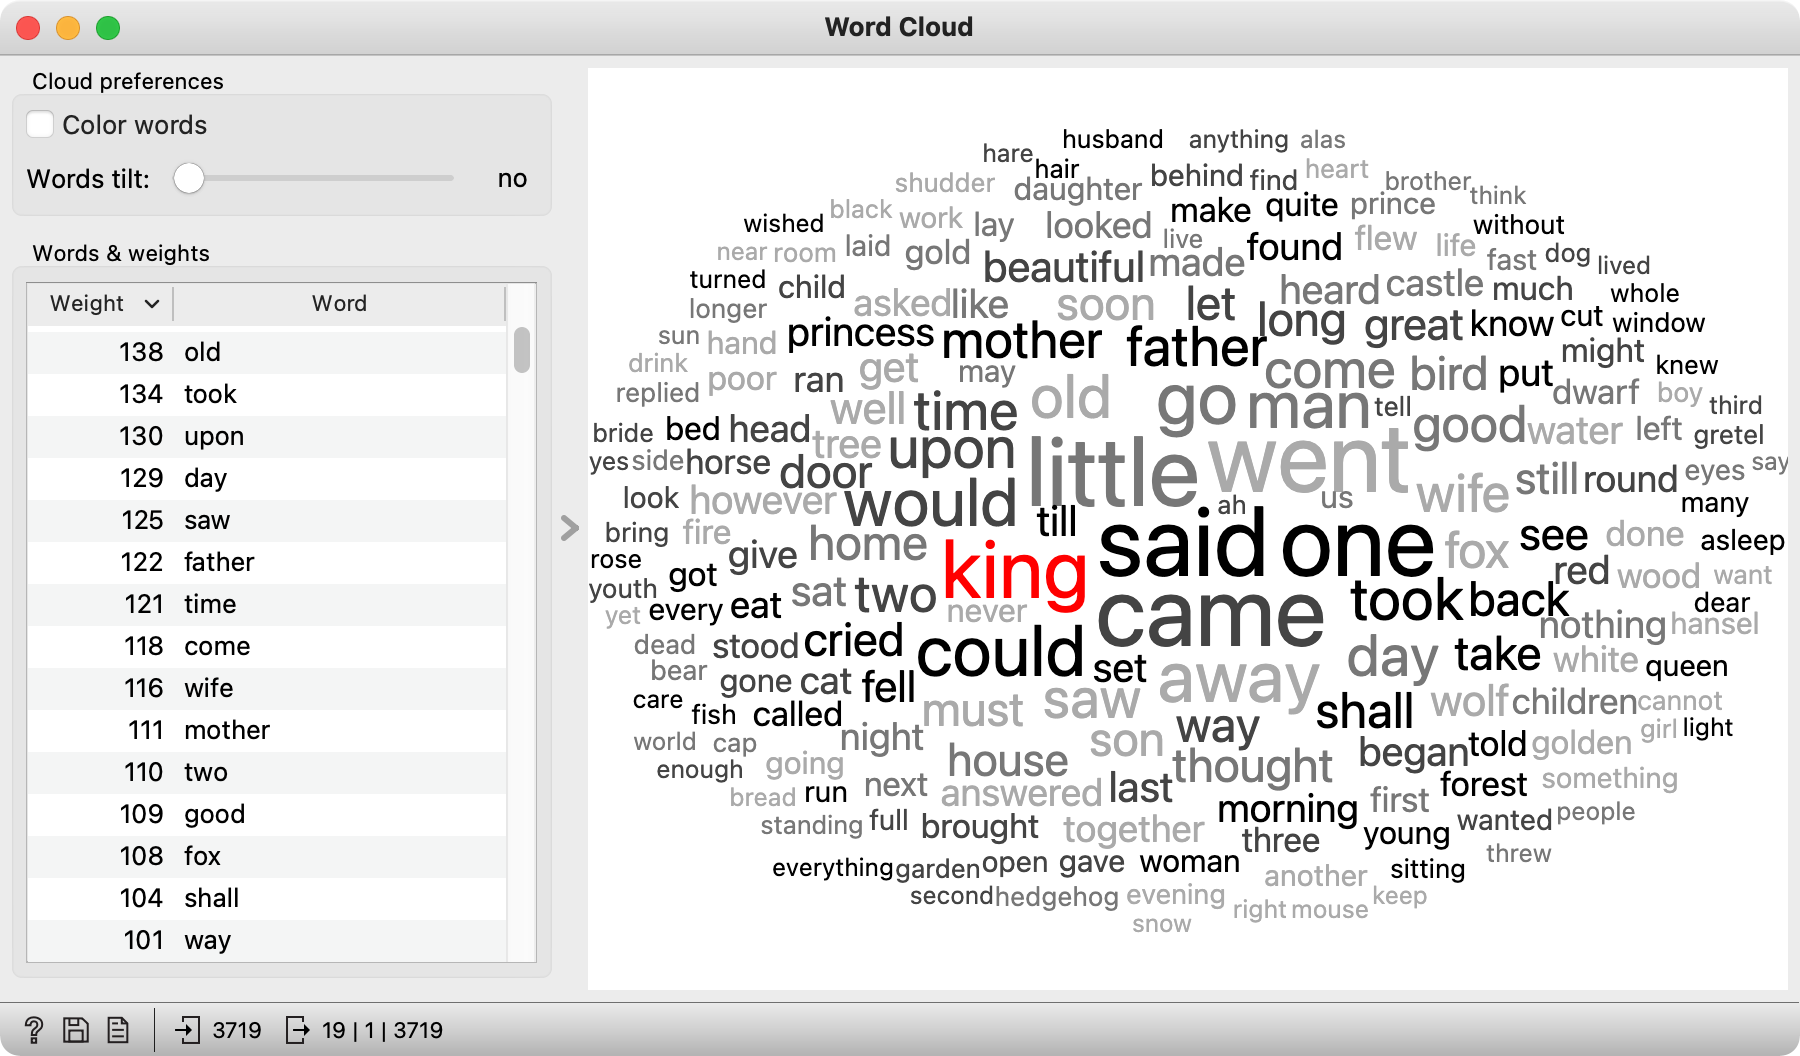
\includegraphics[scale=0.35]{word-cloud.png}}
      \hspace{6cm}
      }
    \caption{$\;$}
\end{figure*}
